%
% File acl20ying a ontact: Maggie Li (cswjli@comp.polyu.edu.hk), Michael White (mwhite@ling.osu.edu)
%%
%% Based on the style files for ACL2008 by Joakim Nivre and Noah Smith
%% and that of ACL2010 by Jing-Shin Chang and Philipp Koehn
\documentclass[10pt,a5paper,twoside]{article}
\usepackage{coling2012}
\usepackage{amsmath}
\usepackage{url}
\usepackage{caption}
\usepackage{subcaption}

\title{Detecting English Writing Styles For Non-native Speakers}

\author{$Rami~Al-Rfou'~~~Yejin~Choi$ \\
  Department of Computer Science \\
  Stony Brook University \\
  NY 11794, USA \\
  \texttt{ \{ralrfou, ychoi\}@cs.stonybrook.edu}}


\begin{document}
\maketitle
\abstractEn{
  Analyzing writing styles of non-native speakers. In this
  paper, we analyze the discussion pages of English Wikipedia which are written by a
  diverse group of users. Using learning algorithms we are able to detect
  native speakers writing style with an accuracy of 74\%. Given the large number
  of languages spoken natively by English Wikipedia users, we measure their similarities
  by comparing the influence they have on English writing style of their
  speakers. Our results show that languages known to have the same origin and
  development path have similar footprint on the English writing style. To
  enable further studies, the dataset we extracted from Wikipedia will be made
  available publicly.
}

\keywordsEn{Stylometric Analysis, Wikipedia, Author attribution, Classification,
Clustering}

\newpage

\section{Introduction}
Stylometric analysis has important applications that cover deception detection, authorship attribution and vandalism detection.
Analyzing writing styles for non-native speakers becomes harder due to the influence of the native language on the usage of the new learned language.
Such influence introduces a bias in the orthographical and syntactic errors made by the author and the choice of vocabulary \cite{koppel2005automatically}.

Previous work focused on smaller datasets like {International Corpus of Learner English} (ICLE) \cite{koppel2005automatically, koppel2005determining, argamon2009automatically}. This choice limits the number of the native languages targeted and the set of topics covered.
It also focuses on features that might only appear in the writing styles of
students, like choice of words \cite{tsur2007using, zheng2003authorship,
gamon2004linguistic}. Syntactic features as subject-verb disagreement, mismatch of noun-number pairs and wrong usage of determiners were studied by \cite{wong2009contrastive}. More sophisticated syntactic features as parse trees were used by examining the frequency of the usage patterns of some distinguishable rules \cite{wong2010parser, wongdras2011EMNLP}.

Different from previous work, we use English Wikipedia talk pages to extract the comments made by the
users. Our dataset is more challenging to study for the following reasons:
First, the comments tend to be shorter in length than the articles written by
students learning English. Second, Wikipedia users represent more diverse
spectrum of skills and the articles cover a wider range of topics. Moreover, the
style of the comments is more conversational and loosely following proper English
grammar. Finally, the number of the languages targeted is larger.

This paper is structured as follows. Section \ref{wiki} discusses various
aspects of Wikipedia's structure and content. Section \ref{setup} describes
the methodologies used to construct the dataset and filter the noise. In section
\ref{features} we explain the features used in the following experiments.
Section \ref{exps} discusses the results of the three major experiments conducted.
Finally, we discuss our conclusions and possible venues of future work.

\section{Wikipedia}
\label{wiki}
Wikipedia is the de facto source of knowledge for internet users. Recently, it
is has been extensively used to help solving different information retrieval
tasks, especially the ones that involves semantic aspects \cite{Milne08aneffective}.
The use of Wikipedia can be expanded to help the
 common NLP tools to perform better; the size of the data and the diversity of
 authors and topics plays a key role. Moreover, the sustained growth of Wikipedia
 content of can bring performance gains with no much additional complexity costs.

With more than 90 thousand active users and 4.4 million article in its English
version, the content of Wikipedia spans large number of topics. The diversity
of authors beside the recorded versions that are stored in the database presents
an interesting source of written language usage. Such resource presents a higher quality of data that is not achievable by the other commonly used sources of text as news, blogs and scientific articles.

Such successful website has a complex database structure to serve its users.
Therefore, extracting data is not trivial. Our goal is to identify the
languages skills of the users and collect their contributions. To achieve the
first task, Wikipedia has an information box called \emph{Babel} that users can
add voluntarily to their profile pages to state their skills in different
languages. A user can identify her native language
and her skills in non-native languages on a scale of 0-5.

The task of collecting the contributions of a specific user is a more complex
procedure. The diffs between Wikipedia pages revisions has to be generated and
linked back to the user table. The resources we have are not sufficient enough to process such
huge amount of data\footnote{Recent efforts were
made to generate the diffs \url{http://dumps.wikimedia.org/other/diffdb/}}.
Instead we noticed that Wikipedia pages have accompanying discussion pages where
users discuss different aspects of the articles. In those pages, the style
guideline encourages the user to sign her comments with her own signature that
links back her user page. The style of writing of those
talk pages are less formal and technical than the main pages of Wikipedia and has more conversational stylistic features.

\section{Experimental Setup}
\label{setup}
In English Wikipedia, we found that around 60 thousands users specified their language skills, 47\% of
them are English native speakers. The total number of comments found in the
processed talk pages is around 12 million comment. Only 2.4 million comment has users with identified language skills. As not all the users contributes to the talk pages, the number of users who makes at least one comment in the extracted comments is around 30 thousand user.

Since we have large number of comments and users, we have to filter the user
base to increase the quality of the gathered data. The following is the
description of the rules that were applied:
\begin{compactitem}
\item Only the users of the most frequent 20 native languages are considered.
\item English native speakers can pick more fine grained categories. Only
  speakers under the US English native category are selected. This decision was made to avoid the
  variations of English writing style among different dialects and countries. Moreover,
  this step helps us to filter the non-native speakers who are proficient in
  English so they chose the general Native English category for their skills
  instead of specifying their skill to be at level 5 fluency at English.
\item Users who specified more than one native language are excluded. To help
  us to avoid improbable scenarios where users claim to be native in many
languages.
\end{compactitem}

The dataset after filtering the users is now composed of 9857 user and 589228
comments. Comments were filtered according to the following criteria:
\begin{compactitem}
\item The accepted comments have to have at least 20 tokens.
\item Proper nouns are replaced by their tags to avoid bias toward topics.
\item Non-ASCII characters are replaced by a special character to avoid bias
toward non-English characters usage in the comments.
\item The classifier has balanced number of comments for each of its classes.
  Therefore, the two baseline classifiers; the most common label and the random
  classifier will have an accuracy of \verb+1/(number of classes)+.
\item The data set is split to 70\% training set, 10\% development set and 20\%
as a testing set.
\end{compactitem}

\section{Experiments}
\subsection{Features}
\label{features}
Given a training dataset, the comments are grouped by their class to construct
frequency distribution of the following n-grams:
\begin{compactitem}
\item 1-4 grams over the comments' words.
\item 1-4 grams over the comments' characters.
\item 1-4 grams over the part of speech tags of comments' words.
\end{compactitem}
For each class we will construct $3*4$ n-gram models. For each comment in the
testing data we will construct a feature vector of the similarity scores between
the comment and each n-gram models for every class. Therefore, if a problem has six
classes, this will generate $6*3*4 = 72$ features for each comment.

For example, the similarity scores ($Sim$) calculated for a comment ($C$)
against the words n-grams models $words\_model(n)$.

\[
  count(x, n) = \left\{
  \begin{array}{l l}
    words\_model(n, word), & \\\quad \text{if $x$ is in $words\_model(n)$}\\
    1,&\\\quad \text{if $x$ is not seen before}\\
  \end{array} \right.
\]
\[
  Sim(C, n) = \sum_{x \in ngrams(C,n)} \log_2 (count(x, n))
\]

Other features are also include the relative frequency of each of the stop words
mentioned in the comment. The 125 stop words are extracted from the NLTK stop
words corpus\cite{nltk}. Moreover, the average size of words, the size of the
comments and the average number of sentences are also included.

\subsection{Native vs Non-native Experiment}
\label{exps}
This experiment aims to detect the non-native speakers writing styles. The
classifier should be able to distinguish between comments by native speakers
and other non-native speakers.
All users with native language other than English are placed into one category.
The number of comments used is around 322K comment. Table
\ref{table:results} shows that the linear SVM classifier succeeds to reach
$74.53\%$ accuracy given the features explained in section \ref{features}.
\begin{table}
  \begin{center}
  \begin{tabular}{l|ll}
	Experiment & Logistic Regression & Linear SVM
	\\\hline
	Non-native & 74.45\% & 74.53\%\\
	Frequent & 50.27\% & 50.26\%\\
	Families & 50.81\% &50.53\% \\
\end{tabular}
\caption{Accuracy of classification using different learning algorithms.}
\label{table:results}
\end{center}
\end{table}

The most informative features are words trigrams, words uni-gram, words bi-gram,
words 4-gram, characters bigrams, POS tags 4-grams, ordered by their importance.
Table \ref{table:nonnative} shows the most correlated grams with (non) native
speakers.

Analyzing the table \ref{table:nonnative}, we can notice that some of the n-grams
indicate common grammatical mistakes in the non-native speakers writing styles.
For example, words unigrams show that non-native speakers tend to use earth
instead of Earth. Characters bigram shows that separating the comma from the
previous word by a space is a common usage of punctuation for non-native speakers.
The usage of articles is a problematic issue for non-native speakers, in the
words 4-grams we can see using the article \emph{the} before a proper noun is
frequent pattern, this trend of using \emph{the} more than needed can be confirmed by the characters bigrams where \emph{th} appears. Word trigram shows that native speakers use \emph{the} correctly in \emph{in the middle} where we expect non-native speakers to use \emph{in middle}.
Moreover, from the characters bigrams non-native speakers use \emph{at} less
than the native speakers which could suggest that they misuse the other articles
where \emph{at} should be used. Characters bigrams shows a trend in spelling
mistakes, where non-native speakers type single \emph{l} instead of \emph{ll}.
Another spelling usage trend is the less frequent usage of apostrophes \emph{'},
this can be traced by more frequent usage of \emph{am} in words unigrams for non-native speakers and the appearance of \emph{don't} in the words 4-grams for native speakers.

\begin{table}[t]
  \begin{subtable}[]{0.5\textwidth}
    \begin{tabular}{l|ll|}
     \textbf{Feature} & \textbf{Speaker}  & \textbf{Gram}
     \\\hline
     Words & Non&article on NNP\\
     Trigrams& Native&  \emph{comma} you have\\\cline{2-3}
             & Native& used in the\\
             &  &in the middle\\\hline
       Words &Non& scene, To,\\
     Unigrams&Native&describing, earth,\\\cline{2-3}
             && referenced, am\\\hline
      Words  &Non& You have, we do\\
      Bigrams&Native& of people\\\cline{2-3}
             &Native& years of, I see\\
             &&if you\\\hline
       Words &Non& but I think that\\
     4-grams  &Native&by the NNP of\\\cline{2-3}
              &&( or at least\\
              &Native&NNP on NNP NNP\\
              &&if you don't\\\hline
    Characters&Non& th, e \emph{space},\\
         Bigrams &Native& \emph{space} \emph{comma}\\ \cline{2-3}
                 &Native& l-, at, ll\\\hline
      PoS 4-gram &Non& NNS \textbf{,} DT NN\\
                 &Native& MD VB VBN \textbf{,}\\\cline{2-3}
                 &Native& \textbf{,} PRP VBZ JJ\\
                 && VBP NN IN NN\\
      \end{tabular}
    \label{table:nonnative}
    \caption{Non-native speakers experiment}
  \end{subtable}
  \begin{subtable}[]{0.5\textwidth}
   \begin{tabular}{l|ll}
    \textbf{Feature} & \textbf{Speaker}  & \textbf{Gram}
   \\\hline
   Words & Russian &prove that\\
    Bigrams& German& you leave\\
    & Spanish& to reveal\\
    & Dutch & reliance on\\\hline

   Words &Dutch& refuting\\
      Unigrams&Spanish&timelines\\
       &German& tie\\\hline

   Words&Russian& stick to what\\
   Trigrams&Spanish& find out the\\
   &Dutch& end up in\\\hline

   Characters &French& hee \emph{space}\\
   4-grams      &French&ownr\\
&Dutch&c/es\\
   \hline
   Words &French& NNP as far as\\
   4-grams &German& the NNP who\\
   &Spanish& ,etc),\\
   &EN-US& Does anyone know if\\\hline
   PoS 4-gram &Dutch& RB CD -RRB- IN \\
   &EN-US& VBD , RB DT\\
   &EN-US& CD VBD NNS IN\\
   && \\
   && \\
   && \\
   \end{tabular}
   \label{table:frequent}
   \caption{Most frequent languages experiment}
   \end{subtable}
\caption{Correlated grams and speakers. For each class and each informative
features the z-scores of each n-gram are calculated. The n-grams with the
highest z-scores are reported in the table.}
\end{table}

The more fluent the speaker is in English the closer his/her writing
style to the native speaker style. To test our basic intuition,
we have to take advantage of the specific language fluency levels that the speaker can choose
from the available Wikipedia Babel box categories. We designed two different
variations of the previous experiment. In the first we limited
the non-native speakers category to the speakers with basic skills in English,
those who correspond to levels 0-2.
While the second is composed of the more advanced non-native speakers with
English levels ranging from 3-5.
Figure \ref{fluency} shows the classifier error rate in the three previous
variations.

\begin{figure}
\centering
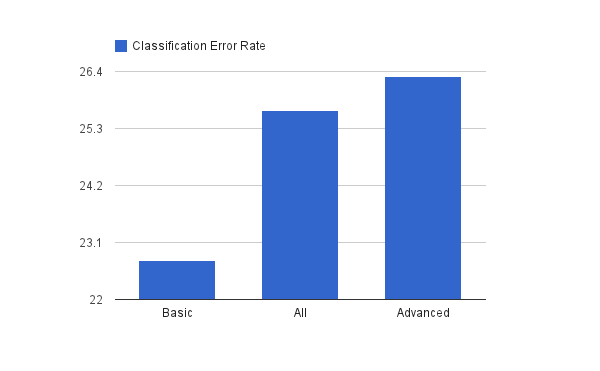
\includegraphics[scale=0.50]{fluency.png}
\caption{Classification error rate against non-native speakers with different
skills.}
\label{fluency}
\end{figure}

The increase of the error rate of classification confirms our intuition.
Moreover, it increases our confidence in the information the users mention in
their profiles regarding their language skills.

\subsection{Frequent Languages Experiment}
\label{frequent}
This experiment aims to classify the comments written by the speakers of the most frequent native languages.
Six languages are selected US-EN, German, Spanish, French, Russian and Dutch.
Figure \ref{pop_cfm} shows the confusion matrix of the logistic regression
classifier.
Table \ref{table:results} shows that the best accuracy that the classifier
achieved is 50.27\% with 150K comment used. We can see clearly that the
Russian users are the easiest to identify. Moreover, the classifier is mostly
confused distinguishing the German and the Dutch users with error $>2.0\%$ and
to a less degree between (EN-US, French). These numbers confirm a basic
intuition that the languages that have geographical proximity will have more
borrowed words and grammars between them. Accordingly this will affect their speakers writing styles in English.

\begin{figure}

\begin{subfigure}[]{0.5\textwidth}
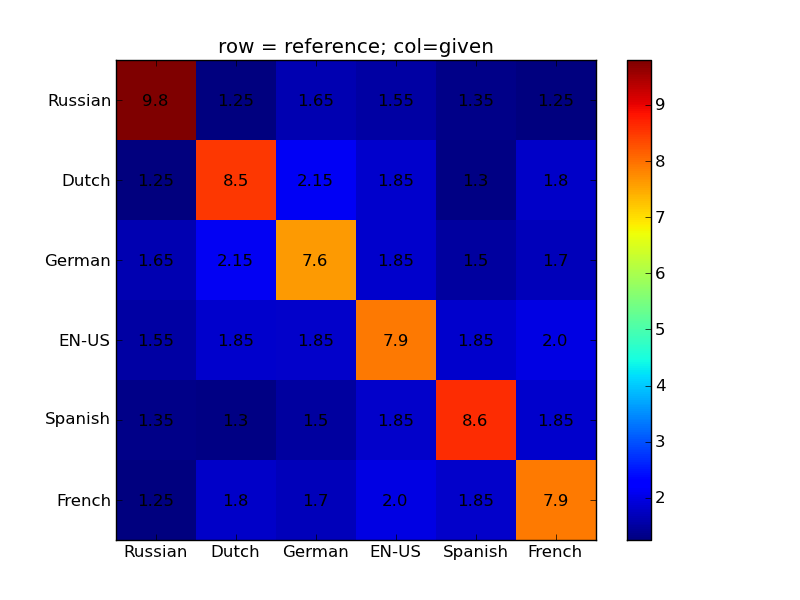
\includegraphics[scale=0.4]{popular_cfm.png}
\caption{Frequent languages experiment}
\label{pop_cfm}
\end{subfigure}
\begin{subfigure}[]{0.5\textwidth}
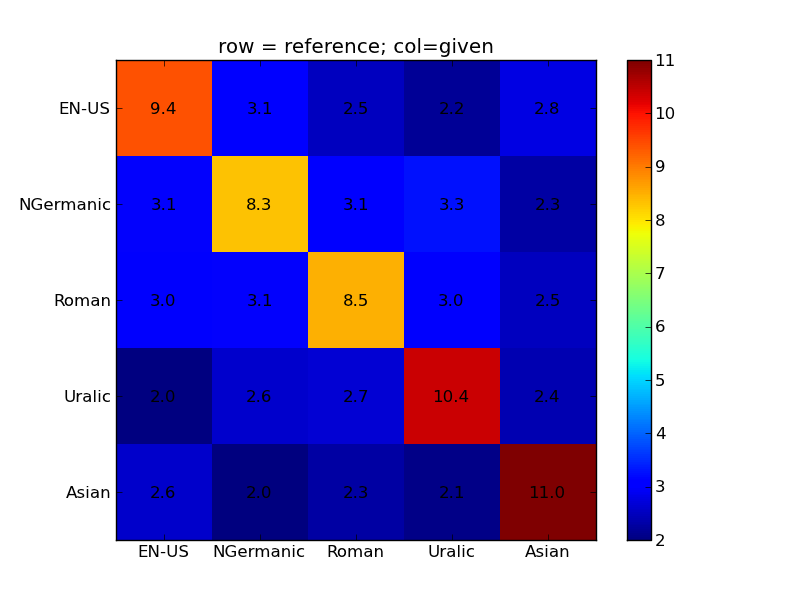
\includegraphics[scale=0.4]{family_cfm.png}
\caption{Languages families}
\label{fam_cfm}
\end{subfigure}

\caption{Confusion Matrices of different Experiments}
\end{figure}

The most informative features are ordered as the following, words bigrams, words
unigrams, words trigrams, characters 4 grams, words 4 grams, POS tags 4-grams.
We can see that the features of the longer grams become less informative once we
increased the number of classes given to the classifier because of sparsity.
It may also indicate the influence of the topic of the comment on the
classification. Table \ref{frequent} shows some different mistakes made by
different native speakers. For example, for French speakers ownr was a common
mistake and not adding the space after the comma was another Spanish speakers
mistake.

\subsection{Languages Families Experiment}

Looking at experiment \ref{exps}, the confusion in classifying Dutch and German
users suggests that there is a similarity between groups of languages. Referring
to the linguistics research history of classifying the languages into families
according to similar features and development history, this experiment tries to
put such grouping under the microscope. The following 18 languages are grouped into 5 families as:
\begin{compactitem}
\item \textbf{Germanic}: German, Dutch, Norwegian, Swedish, Danish.
\item \textbf{Romanace}: Spanish, French, Portuguese, Italian.
\item \textbf{Uralic}: Finnish, Hungarian.
\item \textbf{Asian}: Mandarin, Cantonese, Japanese, Korean.
\item \textbf{Slavic}: Russian, Polish
\end{compactitem}

Figure \ref{fam_cfm} shows that the Slavic and Asian native speakers has a clear style of writing English that is easy to detect relatively. The highest confusion in classification is between the Germanic and Romance languages, where geographical proximity plays a role in similarity. With the same reasoning we can see the confusion between Germanic and Uralic languages.


Taking the opposite approach, we took the speakers of the most frequent 20
native languages and applied the same classification procedure over the new
classes. The accuracy of the classifier is 25\%. However, considering the
confusion matrix as a similarity matrix, we applied the affinity propagation
clustering algorithm \cite{sklearn} over the confusion matrix and the clusters
that were formed are the following:
\begin{compactitem}
\item \textbf{Cluster 1}: Arabic.
\item \textbf{Cluster 2}: Danish, Dutch, Finnish, Norwegian, Swedish.
\item \textbf{Cluster 3}: French, Italian, Portuguese, Spanish.
\item \textbf{Cluster 4}: Mandarin, Cantonese, Japanese, Korean.
\item \textbf{Cluster 5}: Russian, Polish, Turkish.
\item \textbf{Cluster 6}: Hungarian, German, US-EN.
\end{compactitem}

The above clusters support to large extent the literature classification of
languages. Scrutinizing the 4-grams POS tags reveals more interesting
observations regarding non-native speakers usages for English. For example,
in Portuguese speakers comments the pattern \verb+IN DT NN PRP+ appears 0.13\%
of the total number of their comments POS 4-grams. However, it only appears
0.04\% in the Korean speakers comments. Another notice can be detected by
looking at the \verb+NN NN IN DT+'s usage in Portuguese and Polish comments. It
appears 0.15\% in the former POS 4-grams but only 0.05\% in the later. Arabic
speakers tend to use the pattern \verb+TO DT NN IN+ so frequently that it
appears 0.11\% while it is less than 0.06\% for other speakers POS 4-gram
distributions. Finally, Japanese and Danish speakers slightly prefer the pattern
\verb+NN PRP VBZ RB+ more than others.

\subsection{Learning Algorithms}

Figure \ref{comb_lc} shows a typical over fitting situation where the more data
you have the better the classifier can achieve. And here the size of data that
can be extracted from Wikipedia plays a significant role to boost the accuracy
from 37\% to over 50\% in case of the Frequent languages and Families of
languages experiments. This confirms the importance of the coverage of words in
the language models that supplies the frequency counts on the performance of the classifier.

\begin{figure}[t]
\centering
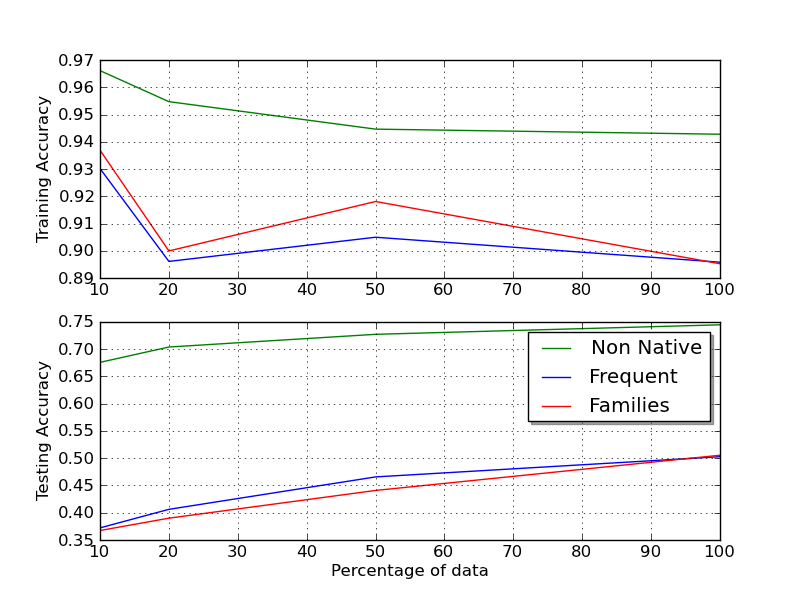
\includegraphics[scale=0.45]{combined_lc.png}
\caption{Learning curves of the logistic regression algorithm.}
\label{comb_lc}
\end{figure}


\section*{Conclusions and Future Work}
\label{conc}
As our results shows promising applications and trends using Wikipedia data to solve hard problems in robust means, there are many paths to improve our results and discover more interesting insights.

Moreover, as the learning curves show, it worth the effort increasing the size
of the data in order of magnitude by adding the Wikipedia diffs, especially the
non minor ones, as it represents another source of users' contributions. Moreover, the minimum size of the comments affects the performance of our classifiers, the relation between the quality of the data used and the accuracy of the classification is another interesting aspect.

The languages families experiments suggest the usefulness of using the English
writing styles to define the similarities between different languages. This
could lead to an interesting explanations and/or observations regarding the
origins of some languages as Korean language which is still a controversial topic.

Another direction is to solve the over fitting problem in our learning algorithms by applying smarter feature selection and adding more distinguishing features.

\section*{Acknowledgements}
We would like to thank Steven Skiena and Yanqing Chen for the discussion and the advice.
We are also indebted to the NLTK and the Sklearn teams for producing excellent
NLP and machine learning software libraries.

\bibliography{myrefs}{}
\bibliographystyle{apa}

\end{document}
